\documentclass[10pt]{amsart}
\usepackage{amsmath}
\usepackage{csquotes}
\usepackage{enumitem}
\usepackage{multicol}
\usepackage{tikz}
\usepackage{pgfplots}
\usepackage{caption}
\usepackage{lipsum}
\usepackage[margin=1in]{geometry}
\pgfplotsset{width=10cm,compat=1.9}

\newenvironment{Figure}
{\par\medskip\noindent\minipage{\linewidth}}
{\endminipage\par\medskip}

\newcommand{\R}{\mathbb{R}}

\title{Mathematics and Machine Learning}
\author{Arden Rasmussen}
\date{\today}

\begin{document}
\maketitle

\begin{abstract}
  Machine Learning is a rapidly expanding subject of much research. There are
  many different approaches to the subject of machine learning, and many more
  which are still being researched. This paper provides a short introduction to
  two methods that can be utilized for machine learning. We will focus
  specifically on the mathematics of these methods, and how they are can be used
  for construction artificial intelligence. We will focus on the methods of
  \textit{neural networks} and \textit{genetic algorithms}. These two methods
  can be used in complement together to develop advanced algorithms.
\end{abstract}

\begin{multicols}{2}
  \section{Introduction}%
  \label{sec:introduction}

  \section{Neural Networks}%
  \label{sec:neural_networks}

  A neural network is a computer model that is constructed to emulate the
  biological process of neural networks in brains. These models have been a key
  point for a lot of modern research, and breakthroughs in artificial
  intelligence. This section will attempt to construct an understanding of a
  basic type of neural network. This type of network is formally classified as a
  \textit{Multi Layer Perceptron}.

  \subsection{Structure}%
  \label{sub:structure}

  \subsubsection{Neuron}%
  \label{ssub:neuron}

  The most basic component of a neural network is the \textit{neuron}. A single
  neuron takes input from many sources and produces a single output value. A
  single neuron takes inputs from other neurons or from external sources. For
  each input value the neuron assigns a weight associated with how important
  that value is relative to the other inputs. Then the neuron applies a
  function $f$, to the weighted sum of the input values.

  \begin{Figure}
    \begin{center}
      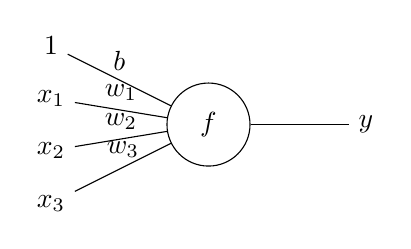
\begin{tikzpicture}[scale=1, transform shape]
  \node (i0) at (-2.0,-1.0) {$x_3$};
  \node (i1) at (-2.0,-0.33) {$x_2$};
  \node (i2) at (-2.0,0.33) {$x_1$};
  \node (i3) at (-2.0,1.0) {$1$};

  \node[circle,draw=black,fill=white,minimum size=3.0em] (n) at (0.0,0.0) {$f$};

  \node (o) at (2.0, 0.0) {$y$};

  \draw (i0) -- node[above] {$w_3$} (n);
  \draw (i1) -- node[above] {$w_2$} (n);
  \draw (i2) -- node[above] {$w_1$} (n);
  \draw (i3) -- node[above] {$b$} (n);

  \draw (n) -- (o);
\end{tikzpicture}

    \end{center}
    \captionof{figure}{A single neuron acting on inputs with provided weights
    $w_i$.}
    \label{fig:nn_single}
  \end{Figure}

  In figure \ref{fig:nn_single}, we see that the neuron takes in four inputs,
  $x_1,\ldots,x_3,1$. Then for each input there is an associated "importance"
  to that input with respect to the other inputs $w_1,\ldots,w_3,b$. This value
  is the weight of that input. The neuron takes the inputs and the weights of
  the inputs and applies the function $f$ on the weighted sum of the inputs
  \begin{align*}
    f(w_1x_1+w_2x_2+w_3x_3+b).
  \end{align*}
  We can then generalize this formula for any number of input neurons to be
  \begin{align}\label{eq:nn_neuron}
    f\left(\sum_{i=1}^Nw_ix_i+b\right).
  \end{align}
  The output of this neuron is either passed along to other neurons as inputs,
  or is the output of our network, and is given to the user.

  The function $f$ that the neuron applies to the weighted sum is called the
  \textit{activation function}. The activation function is a non-linear
  function used to introduce non-linearity into the neural network. Without the
  non-linearity then the network would be just a bunch of linear operations,
  which could be represented as a single matrix, by the introduction of the
  non-linearity we enforce that there must be many steps. This will increase
  the ability of the network to do more complex operations in the future. We
  will go into further detail on activation functions in a different section.

  There are three main \textit{types} of neurons that we will consider.
  \begin{description}
    \item[Input Neurons] Input neurons take information from external inputs,
      such as image data, and then passes that data on to the other neurons in
      the network. The input neurons do no computation, they just pass on their
      information to later neurons.
    \item[Hidden Neurons] Hidden neurons have no connection directly to input
      or output data. They only have what is provided to them from their
      previous layer, and preform the computation that was explained in section
      \ref{sub:neuron}. Then the output value is passed on, either to more
      hidden neurons or to the output neurons.
    \item[Output Neurons] The output neurons are responsible to taking the
      values passed to them by the previous layer of neurons and processing the
      values into an understandable interpretation, such as a probability. They
      then return that data to the user.
  \end{description}
  We will uses these three types of neurons to construct the neural network.

  \subsubsection{Activation Function}%
  \label{ssub:activation_function}

  Activation functions are a method to cause some non-linearity. This
  importance comes into play when we have multiple neurons connecting into one
  another. Since each neuron individually is linear, then this connection of
  neurons will also be linear. That would mean that it could all be modeled as a
  single neuron. This is the reason as to why we need to impose the activation
  functions, to cause non-linearity in between the different neurons, so that
  the function as a whole is not linear. This means that each neuron can be
  trained to be important in the network.

  There are a number of common functions that are used for the activation
  functions. \textit{Sigmoid}, \textit{tanh}, \textit{ReLU}, and other
  variations on \textit{ReLU}. We will describe each of these possible
  activation functions in more detail below. Through usage, it has been found
  that a good default is to use \textit{ReLU}.

  \begin{description}
    \item[Sigmoid] The sigmoid activation function is defined as
      \begin{align*}
        f(x)=\sigma(x)=\frac{1}{1+e^{-x}}.
      \end{align*}
      \begin{Figure}
      \begin{center}
      \begin{tikzpicture}[scale=0.6]
        \begin{axis}[axis lines=center]
          \addplot[]{1/(1+e^(-x))};
        \end{axis}
      \end{tikzpicture}
      \end{center}
      \captionof{figure}{$\frac{1}{1+e^{-x}}$}
      \label{fig:sigmoid}
      \end{Figure}
      The sigmoid function takes any value input to it and squashes it into the
      range of $(0,1)$. However, there are some issues that arise with the
      sigmoid activation function. If the input is small or large, then the
      output becomes saturated, and the gradient of the function at those
      points is zero. This becomes an issue later when using back propagation.
      The other issue is that the output is not centered at zero, this will
      again cause issues later with back propagation.

    \item[tanh] The tanh activation function is similar to the sigmoid
      function, but is constructed to be zero centered. It is defined as
      \begin{align*}
        f(x)=\tanh(x)=\frac{e^x-e^{-x}}{e^x+e^{-x}}.
      \end{align*}
      \begin{Figure}
      \begin{center}
      \begin{tikzpicture}[scale=0.6]
        \begin{axis}[axis lines=center]
          \addplot[]{(e^x-e^(-x))/(e^x+e^(-x))};
        \end{axis}
      \end{tikzpicture}
      \end{center}
      \captionof{figure}{$\frac{e^x-e^{-x}}{e^x+e^{-x}}$}
      \label{fig:tanh}
      \end{Figure}
      The tanh function has the same issue as with the sigmoid function in that
      it can become saturated at large or small values, thus taking the
      gradient to zero. However, this does solve the issue with the zero
      centering. The output of this function will be zero centered.

    \item[ReLU] The ReLU is an acronym for Rectified linear unit. This is
      commonly the default activation function. It is defined as
      \begin{align*}
        f(x)=\max(0,x)=\begin{cases}
          0\quad\text{for}\quad x<0  \\ x\quad\text{for}\quad x\geq 0
        \end{cases}.
      \end{align*}
      \begin{Figure}
      \begin{center}
      \begin{tikzpicture}[scale=0.6]
        \begin{axis}[axis lines=center]
          \addplot[domain=-5:0]{0};
          \addplot[domain=0:5]{x};
        \end{axis}
      \end{tikzpicture}
      \end{center}
      \captionof{figure}{$\max(0,x)$}
      \label{fig:tanh}
      \end{Figure}
      The ReLU function runs into many of the same issues as the other
      activation functions. First it is possible to the neuron to "die" if the
      input is less than zero, then the derivative will be zero, and that
      neuron is effectively dead. This can be very bad in training. It is also
      not zero centered, just like the sigmoid function. However both of these
      issues are usually left to the neural network to deal with, then the
      speed increase that is provided by the simplicity of the function makes
      this significantly better than the other possibilities. This is so much
      faster because there are no computationally expensive computations in the
      function, so it allows the network to execute much faster. It has also
      been shown that using ReLU allows networks to converge faster than other
      activation functions.
  \end{description}

  \subsubsection{Layer}%
  \label{ssub:layer}

  Neural networks are organized into layers. Each layer contains a single type
  of neuron, and can only interact with the layer before it and the one after
  it.

  \begin{Figure}
  \begin{center}
    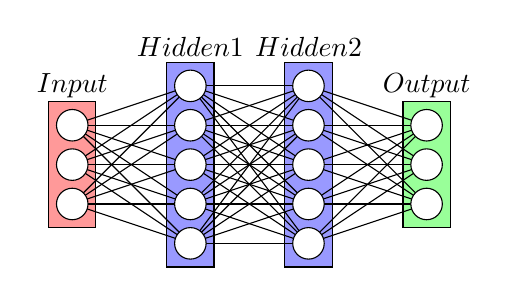
\begin{tikzpicture}[scale=1, transform shape]
  \node (i0) at (0.0,-0.5) {};
  \node (i1) at (0.0,0.0) {};
  \node (i2) at (0.0,0.5) {};

  \node (h00) at (1.5,-1.0) {};
  \node (h01) at (1.5,-0.5) {};
  \node (h02) at (1.5,0.0) {};
  \node (h03) at (1.5,0.5) {};
  \node (h04) at (1.5,1.0) {};

  \node (h10) at (3.0,-1.0) {};
  \node (h11) at (3.0,-0.5) {};
  \node (h12) at (3.0,0.0) {};
  \node (h13) at (3.0,0.5) {};
  \node (h14) at (3.0,1.0) {};

  \node (o0) at (4.5, -0.5) {};
  \node (o1) at (4.5, 0.0) {};
  \node (o2) at (4.5, 0.5) {};

  \node (i) at (0.0,1.0) {$Input$};
  \node (h0) at (1.5,1.5) {$Hidden 1$};
  \node (h0) at (3.0,1.5) {$Hidden 2$};
  \node (i) at (4.5,1.0) {$Output$};

  \filldraw[fill=red!40!white] (-0.3,-0.8) rectangle (0.3, 0.8);

  \filldraw[fill=blue!40!white] (1.2,-1.3) rectangle (1.8, 1.3);
  \filldraw[fill=blue!40!white] (2.7,-1.3) rectangle (3.3, 1.3);

  \filldraw[fill=green!40!white] (4.2,-0.8) rectangle (4.8, 0.8);

  \draw (i0) -- (h00);
  \draw (i0) -- (h01);
  \draw (i0) -- (h02);
  \draw (i0) -- (h03);
  \draw (i0) -- (h04);

  \draw (i1) -- (h00);
  \draw (i1) -- (h01);
  \draw (i1) -- (h02);
  \draw (i1) -- (h03);
  \draw (i1) -- (h04);

  \draw (i2) -- (h00);
  \draw (i2) -- (h01);
  \draw (i2) -- (h02);
  \draw (i2) -- (h03);
  \draw (i2) -- (h04);

  \draw (h00) -- (h10);
  \draw (h00) -- (h11);
  \draw (h00) -- (h12);
  \draw (h00) -- (h13);
  \draw (h00) -- (h14);

  \draw (h01) -- (h10);
  \draw (h01) -- (h11);
  \draw (h01) -- (h12);
  \draw (h01) -- (h13);
  \draw (h01) -- (h14);

  \draw (h02) -- (h10);
  \draw (h02) -- (h11);
  \draw (h02) -- (h12);
  \draw (h02) -- (h13);
  \draw (h02) -- (h14);

  \draw (h03) -- (h10);
  \draw (h03) -- (h11);
  \draw (h03) -- (h12);
  \draw (h03) -- (h13);
  \draw (h03) -- (h14);

  \draw (h04) -- (h10);
  \draw (h04) -- (h11);
  \draw (h04) -- (h12);
  \draw (h04) -- (h13);
  \draw (h04) -- (h14);

  \draw (h10) -- (o0);
  \draw (h10) -- (o1);
  \draw (h10) -- (o2);

  \draw (h11) -- (o0);
  \draw (h11) -- (o1);
  \draw (h11) -- (o2);

  \draw (h12) -- (o0);
  \draw (h12) -- (o1);
  \draw (h12) -- (o2);

  \draw (h13) -- (o0);
  \draw (h13) -- (o1);
  \draw (h13) -- (o2);

  \draw (h14) -- (o0);
  \draw (h14) -- (o1);
  \draw (h14) -- (o2);

  \filldraw[fill=white] (i0) circle (0.2);
  \filldraw[fill=white] (i1) circle (0.2);
  \filldraw[fill=white] (i2) circle (0.2);

  \filldraw[fill=white] (h00) circle (0.2);
  \filldraw[fill=white] (h01) circle (0.2);
  \filldraw[fill=white] (h02) circle (0.2);
  \filldraw[fill=white] (h03) circle (0.2);
  \filldraw[fill=white] (h04) circle (0.2);

  \filldraw[fill=white] (h10) circle (0.2);
  \filldraw[fill=white] (h11) circle (0.2);
  \filldraw[fill=white] (h12) circle (0.2);
  \filldraw[fill=white] (h13) circle (0.2);
  \filldraw[fill=white] (h14) circle (0.2);

  \filldraw[fill=white] (o0) circle (0.2);
  \filldraw[fill=white] (o1) circle (0.2);
  \filldraw[fill=white] (o2) circle (0.2);
\end{tikzpicture}

  \end{center}
  \captionof{figure}{Example structure of a two layer neural network, with the
  four layers highlighted in different colors.}
  \label{fig:nn_two_layer}
  \end{Figure}

  In figure \ref{fig:nn_two_layer} an example of how each layer of neurons
  interact with one another can be seen. Note how each neuron of the previous
  layer is now an input for every neuron of the current layer. We call this
  type of network a "two layer" network even though it clearly has four layers.
  This is because the input and output layers must always be present, and so it
  is not important if we count them or not, thus the important number is the
  number of hidden layers in the network.

  \subsubsection{Network}%
  \label{ssub:network}

  \subsection{Forward Propagation}%
  \label{sub:forward_propagation}

  \subsection{Learning}%
  \label{sub:learning}

  \subsubsection{Gradient Descent}%
  \label{ssub:gradient_descent}

  \subsubsection{Back Propagation}%
  \label{ssub:back_propagation}

  \subsection{Summary}%
  \label{sub:summary}

  \section{Genetic Algorithms}%
  \label{sec:genetic_algorithms}

  \subsection{Structure}%
  \label{sub:structure}

  \subsubsection{Initialization}%
  \label{ssub:initialization}

  \subsubsection{Evaluation}%
  \label{ssub:evaluation}

  \subsubsection{Selection}%
  \label{ssub:selection}

  \subsubsection{Recombination}%
  \label{ssub:recombination}

  \subsubsection{Mutation}%
  \label{ssub:mutation}

  \subsubsection{Replacement}%
  \label{ssub:replacement}

  \subsection{Integration}%
  \label{sub:integration}

  \subsection{Summary}%
  \label{sub:summaryb}

\end{multicols}

% \begin{multicols}{2}
%   \section{Introduction}%
%   \label{sec:introduction}
%
%   Machine learning is a rapidly developing subject of research. Because of the
%   rapid movement of research, it can be difficult to achieve a base
%   understanding of the methods and topics. We aim to provide an introduction to
%   two basic, but extremely important, concepts of machine learning.
%
%   This paper will provide thorough introduction to each concept, and
%   demonstrate the mathematics behind the method. Then provide a process that
%   could be programmed to construct a functioning implementation of the process.
%
%   \section{Neural Networks}%
%   \label{sec:neural_networks}
%
%   A neural network is a computer model that is constructed to emulate the
%   biological process of neural networks in brains. These models have been a key
%   point for a lot of modern research, and breakthroughs in artificial
%   intelligence. This section will attempt to construct an understanding of a
%   basic type of neural network. This type of network is formally classified as a
%   \textit{Multi Layer Perceptron}.
%
%   \subsection{Neuron}%
%   \label{sub:neuron}
%
%   The most basic component of a neural network is the \textit{neuron}. A single
%   neuron takes input from many sources and produces a single output value. A
%   single neuron takes inputs from other neurons or from external sources. For
%   each input value the neuron assigns a weight associated with how important
%   that value is relative to the other inputs. Then the neuron applies a
%   function $f$, to the weighted sum of the input values.
%
%   \begin{Figure}
%     \begin{center}
%       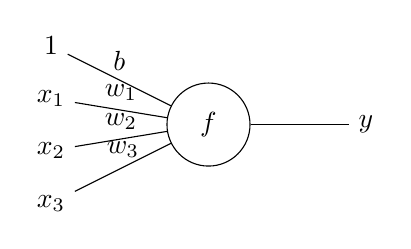
\begin{tikzpicture}[scale=1, transform shape]
  \node (i0) at (-2.0,-1.0) {$x_3$};
  \node (i1) at (-2.0,-0.33) {$x_2$};
  \node (i2) at (-2.0,0.33) {$x_1$};
  \node (i3) at (-2.0,1.0) {$1$};

  \node[circle,draw=black,fill=white,minimum size=3.0em] (n) at (0.0,0.0) {$f$};

  \node (o) at (2.0, 0.0) {$y$};

  \draw (i0) -- node[above] {$w_3$} (n);
  \draw (i1) -- node[above] {$w_2$} (n);
  \draw (i2) -- node[above] {$w_1$} (n);
  \draw (i3) -- node[above] {$b$} (n);

  \draw (n) -- (o);
\end{tikzpicture}

%     \end{center}
%     \captionof{figure}{A single neuron acting on inputs with provided weights
%     $w_i$.}
%     \label{fig:nn_single}
%   \end{Figure}
%
%   In figure \ref{fig:nn_single}, we see that the neuron takes in four inputs,
%   $x_1,\ldots,x_3,1$. Then for each input there is an associated "importance"
%   to that input with respect to the other inputs $w_1,\ldots,w_3,b$. This value
%   is the weight of that input. The neuron takes the inputs and the weights of
%   the inputs and applies the function $f$ on the weighted sum of the inputs
%   \begin{align*}
%     f(w_1x_1+w_2x_2+w_3x_3+b).
%   \end{align*}
%   We can then generalize this formula for any number of input neurons to be
%   \begin{align}\label{eq:nn_neuron}
%     f\left(\sum_{i=1}^Nw_ix_i+b\right).
%   \end{align}
%   The output of this neuron is either passed along to other neurons as inputs,
%   or is the output of our network, and is given to the user.
%
%   The function $f$ that the neuron applies to the weighted sum is called the
%   \textit{activation function}. The activation function is a non-linear
%   function used to introduce non-linearity into the neural network. Without the
%   non-linearity then the network would be just a bunch of linear operations,
%   which could be represented as a single matrix, by the introduction of the
%   non-linearity we enforce that there must be many steps. This will increase
%   the ability of the network to do more complex operations in the future. We
%   will go into further detail on activation functions in a different section.
%
%   \subsection{Multi Layer Perceptron}%
%   \label{sub:multi_layer_perceptron}
%
%   The multi layer perceptron network is a network that contains three types of
%   neurons organized into layers.
%
%   \subsubsection{Neuron Types}%
%   \label{ssub:neuron_types}
%
%   \begin{description}
%     \item[Input Neurons] Input neurons take information from external inputs,
%       such as image data, and then passes that data on to the other neurons in
%       the network. The input neurons do no computation, they just pass on their
%       information to later neurons.
%     \item[Hidden Neurons] Hidden neurons have no connection directly to input
%       or output data. They only have what is provided to them from their
%       previous layer, and preform the computation that was explained in section
%       \ref{sub:neuron}. Then the output value is passed on, either to more
%       hidden neurons or to the output neurons.
%     \item[Output Neurons] The output neurons are responsible to taking the
%       values passed to them by the previous layer of neurons and processing the
%       values into an understandable interpretation, such as a probability. They
%       then return that data to the user.
%   \end{description}
%
%   \subsubsection{Layers}%
%   \label{ssub:layers}
%
%   Neural networks are organized into layers. Each layer contains a single type
%   of neuron, and can only interact with the layer before it and the one after
%   it.
%
%   \begin{Figure}
%   \begin{center}
%     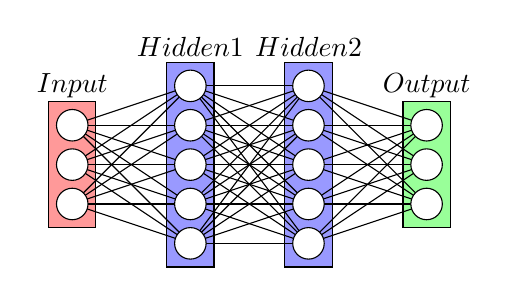
\begin{tikzpicture}[scale=1, transform shape]
  \node (i0) at (0.0,-0.5) {};
  \node (i1) at (0.0,0.0) {};
  \node (i2) at (0.0,0.5) {};

  \node (h00) at (1.5,-1.0) {};
  \node (h01) at (1.5,-0.5) {};
  \node (h02) at (1.5,0.0) {};
  \node (h03) at (1.5,0.5) {};
  \node (h04) at (1.5,1.0) {};

  \node (h10) at (3.0,-1.0) {};
  \node (h11) at (3.0,-0.5) {};
  \node (h12) at (3.0,0.0) {};
  \node (h13) at (3.0,0.5) {};
  \node (h14) at (3.0,1.0) {};

  \node (o0) at (4.5, -0.5) {};
  \node (o1) at (4.5, 0.0) {};
  \node (o2) at (4.5, 0.5) {};

  \node (i) at (0.0,1.0) {$Input$};
  \node (h0) at (1.5,1.5) {$Hidden 1$};
  \node (h0) at (3.0,1.5) {$Hidden 2$};
  \node (i) at (4.5,1.0) {$Output$};

  \filldraw[fill=red!40!white] (-0.3,-0.8) rectangle (0.3, 0.8);

  \filldraw[fill=blue!40!white] (1.2,-1.3) rectangle (1.8, 1.3);
  \filldraw[fill=blue!40!white] (2.7,-1.3) rectangle (3.3, 1.3);

  \filldraw[fill=green!40!white] (4.2,-0.8) rectangle (4.8, 0.8);

  \draw (i0) -- (h00);
  \draw (i0) -- (h01);
  \draw (i0) -- (h02);
  \draw (i0) -- (h03);
  \draw (i0) -- (h04);

  \draw (i1) -- (h00);
  \draw (i1) -- (h01);
  \draw (i1) -- (h02);
  \draw (i1) -- (h03);
  \draw (i1) -- (h04);

  \draw (i2) -- (h00);
  \draw (i2) -- (h01);
  \draw (i2) -- (h02);
  \draw (i2) -- (h03);
  \draw (i2) -- (h04);

  \draw (h00) -- (h10);
  \draw (h00) -- (h11);
  \draw (h00) -- (h12);
  \draw (h00) -- (h13);
  \draw (h00) -- (h14);

  \draw (h01) -- (h10);
  \draw (h01) -- (h11);
  \draw (h01) -- (h12);
  \draw (h01) -- (h13);
  \draw (h01) -- (h14);

  \draw (h02) -- (h10);
  \draw (h02) -- (h11);
  \draw (h02) -- (h12);
  \draw (h02) -- (h13);
  \draw (h02) -- (h14);

  \draw (h03) -- (h10);
  \draw (h03) -- (h11);
  \draw (h03) -- (h12);
  \draw (h03) -- (h13);
  \draw (h03) -- (h14);

  \draw (h04) -- (h10);
  \draw (h04) -- (h11);
  \draw (h04) -- (h12);
  \draw (h04) -- (h13);
  \draw (h04) -- (h14);

  \draw (h10) -- (o0);
  \draw (h10) -- (o1);
  \draw (h10) -- (o2);

  \draw (h11) -- (o0);
  \draw (h11) -- (o1);
  \draw (h11) -- (o2);

  \draw (h12) -- (o0);
  \draw (h12) -- (o1);
  \draw (h12) -- (o2);

  \draw (h13) -- (o0);
  \draw (h13) -- (o1);
  \draw (h13) -- (o2);

  \draw (h14) -- (o0);
  \draw (h14) -- (o1);
  \draw (h14) -- (o2);

  \filldraw[fill=white] (i0) circle (0.2);
  \filldraw[fill=white] (i1) circle (0.2);
  \filldraw[fill=white] (i2) circle (0.2);

  \filldraw[fill=white] (h00) circle (0.2);
  \filldraw[fill=white] (h01) circle (0.2);
  \filldraw[fill=white] (h02) circle (0.2);
  \filldraw[fill=white] (h03) circle (0.2);
  \filldraw[fill=white] (h04) circle (0.2);

  \filldraw[fill=white] (h10) circle (0.2);
  \filldraw[fill=white] (h11) circle (0.2);
  \filldraw[fill=white] (h12) circle (0.2);
  \filldraw[fill=white] (h13) circle (0.2);
  \filldraw[fill=white] (h14) circle (0.2);

  \filldraw[fill=white] (o0) circle (0.2);
  \filldraw[fill=white] (o1) circle (0.2);
  \filldraw[fill=white] (o2) circle (0.2);
\end{tikzpicture}

%   \end{center}
%   \captionof{figure}{Example structure of a two layer neural network, with the
%   four layers highlighted in different colors.}
%   \label{fig:nn_two_layer}
%   \end{Figure}
%
%   In figure \ref{fig:nn_two_layer} an example of how each layer of neurons
%   interact with one another can be seen. Note how each neuron of the previous
%   layer is now an input for every neuron of the current layer. We call this
%   type of network a "two layer" network even though it clearly has four layers.
%   This is because the input and output layers must always be present, and so it
%   is not important if we count them or not, thus the important number is the
%   number of hidden layers in the network.
%
%   \subsection{Feed Forward}%
%   \label{sub:feed_forward}
%
%   Feed forward is the process of taking the inputs of the network and
%   determining the outputs of the network.
%
%   \begin{Figure}
%   \begin{center}
%     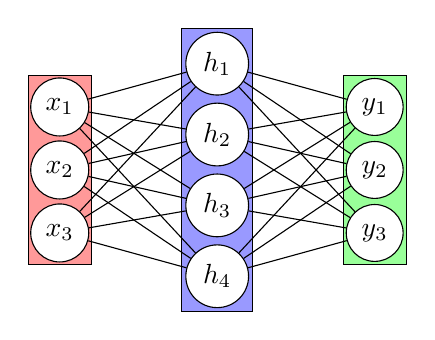
\begin{tikzpicture}[scale=1, transform shape]

  \filldraw[fill=red!40!white] (-0.4,-1.2) rectangle (0.4, 1.2);
  \filldraw[fill=blue!40!white] (1.55,-1.8) rectangle (2.45, 1.8);
  \filldraw[fill=green!40!white] (3.6,-1.2) rectangle (4.4, 1.2);

  \node[circle,fill=white,draw=black] (i1) at (0.0,0.0) {$x_2$};
  \node[circle,fill=white,draw=black] (i0) at (0.0,-0.8) {$x_3$};
  \node[circle,fill=white,draw=black] (i2) at (0.0,0.8) {$x_1$};

  \node[circle,fill=white,draw=black] (h0) at (2.0,-1.35) {$h_4$};
  \node[circle,fill=white,draw=black] (h1) at (2.0,-0.45) {$h_3$};
  \node[circle,fill=white,draw=black] (h2) at (2.0,0.45) {$h_2$};
  \node[circle,fill=white,draw=black] (h3) at (2.0,1.35) {$h_1$};

  \node[circle,fill=white,draw=black] (o0) at (4.0, -0.8) {$y_3$};
  \node[circle,fill=white,draw=black] (o1) at (4.0, 0.0) {$y_2$};
  \node[circle,fill=white,draw=black] (o2) at (4.0, 0.8) {$y_1$};

  \draw (i0) -- (h0);
  \draw (i0) -- (h1);
  \draw (i0) -- (h2);
  \draw (i0) -- (h3);

  \draw (i1) -- (h0);
  \draw (i1) -- (h1);
  \draw (i1) -- (h2);
  \draw (i1) -- (h3);

  \draw (i2) -- (h0);
  \draw (i2) -- (h1);
  \draw (i2) -- (h2);
  \draw (i2) -- (h3);

  \draw (h0) -- (o0);
  \draw (h0) -- (o1);
  \draw (h0) -- (o2);

  \draw (h1) -- (o0);
  \draw (h1) -- (o1);
  \draw (h1) -- (o2);

  \draw (h2) -- (o0);
  \draw (h2) -- (o1);
  \draw (h2) -- (o2);

  \draw (h3) -- (o0);
  \draw (h3) -- (o1);
  \draw (h3) -- (o2);
\end{tikzpicture}

%   \end{center}
%   \captionof{figure}{Example of a one layer neural network.}
%   \label{fig:nn_one_layer}
%   \end{Figure}
%
%   We will use the example displayed in figure \ref{fig:nn_one_layer} for the
%   explanation of the feed forward process. We also make the assumption that
%   each neuron in the layer will use the same activation function $f$.
%
%   Using the equation that we determined for the single neuron
%   \eqref{eq:nn_neuron}, we are able to find the weighted sums for all the
%   neurons in the hidden layer. They are
%   \begin{align*}
%     h_1 &= w_{11}x_1+w_{12}x_2+w_{13}x_3+b_1\\
%     h_2 &= w_{21}x_1+w_{22}x_2+w_{23}x_3+b_2\\
%     h_3 &= w_{31}x_1+w_{32}x_2+w_{33}x_3+b_3\\
%     h_4 &= w_{41}x_1+w_{42}x_2+w_{43}x_3+b_4.\\
%   \end{align*}
%   Where $w_{ij}$ denotes the weight for the $i$th neuron in the hidden layer
%   for the $j$th input neuron value. Similarly $b_i$ denotes the bias term for
%   the $i$th neuron in the hidden layer.
%
%   This system of equations can easily be constructed into a matrix
%   \begin{align*}
%      \begin{bmatrix}
%         h_1\\h_2\\h_3\\h_4
%      \end{bmatrix}=
%      \begin{bmatrix}
%        w_{11} & w_{12} & w_{13} & b_1\\
%        w_{21} & w_{22} & w_{23} & b_2\\
%        w_{31} & w_{32} & w_{33} & b_3\\
%        w_{41} & w_{42} & w_{43} & b_4\\
%      \end{bmatrix}
%      \begin{bmatrix}
%         x_1\\x_2\\x_3\\1
%      \end{bmatrix}.
%   \end{align*}
%   The process that we just did is often called \textit{vectorization}, because
%   we took the equations and converted them into a vector and matrix based form.
%   This is always done for neural networks, due to the fact that the vectorized
%   operations are often significantly faster than doing everything element by
%   element.
%
%   Then the final step is to apply the activation function to the vectorized
%   form of the weighted sums. For this we must simply do it element by element,
%   so we define
%   \begin{align*}
%     \bar{f}&:\R^n\rightarrow\R^n\\
%     \bar{f}(\vec{x})&=\begin{pmatrix}
%       f(x^1)\\f(x^2)\\ \vdots \\ f(x^n)
%     \end{pmatrix}
%   \end{align*}
%   Then we can simply use the new $\bar{f}$ on the linearized system to get a
%   vector based output. Note that in most cases we leave off the special
%   notation for the vectorized version of $f$ and simply use $\bar{f}=f$.
%
% \end{multicols}

\end{document}
